%=====================================================================
%  IT 7178 Progress Report  -- IEEE Conference format
%  Behaviour-Based Detection of Living-off-the-Land Attacks
%  Olaoluwa E. Sipeolu, Georgia Southern University
%
%  HOW TO USE THIS FILE (read me):
%   * Upload this file, references.bib, and the two figures
%     (fig_provenance_graphs.png, fig_scores.png) to a new Overleaf project.
%   * Set the compiler to pdfLaTeX. Overleaf runs BibTeX automatically.
%   * Sections marked  % >>> WRITE IN YOUR OWN WORDS  contain draft prose or
%     guidance. Paraphrase them in your own voice before submitting so the
%     report reads as yours and passes the AI/plagiarism checks.
%   * Replace every number marked  <<REPLACE>>  with the real value your
%     executed Colab notebook prints from YOUR captured logs.
%=====================================================================
\documentclass[conference]{IEEEtran}
\IEEEoverridecommandlockouts
\usepackage{cite}
\usepackage{amsmath,amssymb,amsfonts}
\usepackage{graphicx}
\usepackage{url}
\usepackage{booktabs}
\usepackage{xcolor}
\def\BibTeX{{\rm B\kern-.05em{\sc i\kern-.025em b}\kern-.08em
    T\kern-.1667em\lower.7ex\hbox{E}\kern-.125emX}}

\begin{document}

\title{Behaviour-Based Detection of Living-off-the-Land Attacks Using
Process and System-Call Provenance Telemetry}

\author{\IEEEauthorblockN{Olaoluwa E. Sipeolu}
\IEEEauthorblockA{\textit{M.S. Information Technology (Cybersecurity)} \\
\textit{Georgia Southern University}\\
Statesboro, GA, USA \\
Course: IT 7178}}

\maketitle

%---------------------------------------------------------------------
% ABSTRACT -- carried over from your proposal (your own words). Update the
% final two sentences once your results are in so it reflects what you found.
%---------------------------------------------------------------------
\begin{abstract}
Living-off-the-Land (LotL) attacks abuse trusted, pre-installed system
binaries (e.g., PowerShell, WMI, certutil) to execute malicious activity
while evading signature-based defenses, since no foreign malware is
introduced. Existing detectors rely heavily on static indicators or
individual command patterns and struggle to separate malicious binary use
from the frequent benign use of the same tools by administrators. This work
presents a behaviour-based detection framework that models the provenance
context of process execution---parent--child lineage, inter-process
relationships, and sequences of system calls---rather than isolated
commands, so as to distinguish malicious LotL behaviour from legitimate
administrative activity. The approach constructs process-provenance graphs
from host telemetry and derives behavioural features that capture anomalous
execution chains, then applies a transparent scoring model to flag
suspicious sequences. We implement a Linux prototype using \texttt{auditd}
telemetry and evaluate it against benign administrative baselines and
emulated LotL techniques mapped to MITRE ATT\&CK. In this progress report,
preliminary results show that the provenance behaviour score separates
benign and malicious use of identical binaries where a name-based baseline
produces false positives, achieving a precision of \textbf{<<REPLACE>>} and
an $F_1$ of \textbf{<<REPLACE>>} on the current controlled dataset.
\end{abstract}

\begin{IEEEkeywords}
Living-off-the-Land attacks, behaviour-based detection, process provenance,
system-call telemetry, host intrusion detection, MITRE ATT\&CK
\end{IEEEkeywords}

%---------------------------------------------------------------------
\section{Introduction and Motivation}
% >>> This is your draft prose. Keep it; tighten in your own voice.
Modern adversaries increasingly avoid custom malware and instead ``live off
the land,'' repurposing legitimate operating-system utilities to conduct
reconnaissance, privilege escalation, and lateral movement. Because these
binaries are trusted and ubiquitous, allow-listing and signature matching
are ineffective, and the same tools are used constantly by legitimate
administrators, producing high false-positive rates for naive anomaly
detectors~\cite{barrsmith2021survivalism,ongun2021lotl}. The research gap is
a detection approach that reasons over the \emph{behavioural context} in
which a trusted binary executes rather than the binary or command in
isolation. Closing this gap matters because LotL techniques underpin many
high-impact intrusions yet remain difficult to detect without overwhelming
analysts.

This progress report makes three contributions. First, we build a controlled
Linux telemetry lab that captures process-execution provenance for both
benign administrative tasks and emulated LotL techniques. Second, we design
a provenance-graph feature set and a transparent behaviour score that encode
parent--child lineage, obfuscation, and persistence behaviour. Third, we
show a preliminary comparison against a name-based signature baseline that
quantifies the false-positive problem the framework is designed to solve.

% Report organisation
The remainder of this report is organised as follows. Section~II reviews
related work in LotL detection and provenance-based threat detection.
Section~III details the system design, telemetry pipeline, and feature
engineering. Section~IV presents the experimental setup, metrics, and
preliminary results. We conclude with limitations and planned work.

%---------------------------------------------------------------------
\section{Literature Review}
% >>> WRITE IN YOUR OWN WORDS. The paragraphs below summarise real papers
%     with correct citations. Rephrase each summary in your own voice; do not
%     submit this draft text verbatim.

\subsection{Scope of the Review}
We review two bodies of work: (i) detection of LotL and
living-off-the-land-binary (LOLBin) abuse, and (ii) system-level provenance
graphs for host intrusion detection, from which our feature design draws.

\subsection{Detecting LotL and LOLBin Abuse}
Barr-Smith et al.~\cite{barrsmith2021survivalism} performed a large-scale
systematic analysis of Windows malware abusing native binaries, establishing
the prevalence of the LotL problem. Command-level detectors have applied
deep learning to malicious PowerShell~\cite{hendler2018powershell} and
natural-language and active-learning methods to shell command
streams~\cite{ongun2021lotl}, while recent work explores small language
models for command-line obfuscation detection~\cite{liu2328command}. These
approaches largely classify commands in isolation; our work instead models
the execution context around a command.

\subsection{Provenance-Based Threat Detection}
Data provenance reconstructs causal relationships between system entities.
Backtracking intrusions~\cite{king2003backtracking} introduced the idea of
causal dependency graphs for intrusion analysis. SLEUTH~\cite{hossain2017sleuth}
and HOLMES~\cite{milajerdi2019holmes} reconstruct attack scenarios from audit
data in real time, while POIROT~\cite{milajerdi2019poirot} aligns observed
behaviour with known attack graphs for threat hunting. UNICORN~\cite{han2020unicorn}
and ProvDetector~\cite{wang2020provdetector} detect stealthy threats via
whole-system provenance and rare path analysis. To combat alert fatigue,
NoDoze~\cite{hassan2019nodoze} and tactical provenance analysis~\cite{hassan2020rapsheet}
prioritise and triage provenance-derived alerts. Graph-learning methods such
as StreamSpot~\cite{manzoor2016streamspot} and Log2vec~\cite{liu2019log2vec}
embed heterogeneous log/graph structure for anomaly detection. Surveys of the
area~\cite{li2021survey} catalogue these techniques and their trade-offs.

\subsection{Critical Evaluation and Gap}
% >>> WRITE IN YOUR OWN WORDS (a few sentences):
% - Command-only detectors miss context and over-fire on admin use.
% - Full-provenance APT systems are powerful but heavyweight and data-hungry.
% - Gap: a lightweight, interpretable, provenance-aware score aimed
%   specifically at separating benign vs. malicious use of the SAME binaries.
Machine-learning intrusion detection must also contend with the base-rate and
evaluation pitfalls articulated by Sommer and Paxson~\cite{sommer2010outside},
which motivate our emphasis on false-positive behaviour and a transparent,
auditable scoring model.

%---------------------------------------------------------------------
\section{Research Implementation}
% These sections describe YOUR real lab and are factual; light editing is fine.

\subsection{Detailed Approach and Methodology}
Our detection pipeline has four stages: (1) capture process-execution
telemetry with Linux \texttt{auditd}; (2) parse the audit stream into a
process-provenance graph per activity, where nodes are processes and edges
encode parent$\rightarrow$child \texttt{execve} relationships; (3) extract
behavioural features over each graph; and (4) assign a transparent behaviour
score and compare against a name-based baseline. The guiding hypothesis is
that malicious and benign uses of the same trusted binary differ in their
\emph{provenance context}---the launching parent, the surrounding execution
chain, and command-line characteristics---even when the binary itself is
identical.

\subsection{System and Workflow Design}
We built an isolated laboratory using a UTM virtual machine running Ubuntu
Server (ARM64) on an Apple-silicon host. A kernel audit rule records every
\texttt{execve}/\texttt{execveat} system call:
\begin{center}\small
\texttt{-a always,exit -F arch=b64 -S execve,execveat -k lotl\_exec}
\end{center}
A capture harness executes each labelled activity, then extracts the
associated audit records. Benign captures comprise routine administrative
tasks (system inventory, package queries, user/account checks, log review,
and network configuration). Malicious captures emulate LotL techniques,
mapped to MITRE ATT\&CK~\cite{strom2018attack} and modelled on Atomic Red
Team~\cite{atomicredteam} and GTFOBins~\cite{gtfobins}: obfuscated shell
execution via Base64 decoding (T1059.004), ingress-tool-transfer and
download-and-run behaviour (T1105), and cron-based persistence installation
(T1053.003). All emulations are executed safely within the VM.

\subsection{Tools and Technologies}
Telemetry is captured with \texttt{auditd}/\texttt{ausearch}. Parsing,
graph construction, feature extraction, and analysis are implemented in
Python using \texttt{networkx}, \texttt{pandas}, \texttt{scikit-learn}, and
\texttt{matplotlib}. The parser decodes audit records (including hex-encoded
command-line arguments), filters the capture harness itself, and builds one
provenance graph per activity. The behavioural feature set includes
structural features (process count, chain depth, shell-spawns-shell edges),
LotL-binary usage, command-line length and Shannon entropy, and binary
behavioural indicators (Base64-piped-to-shell, hidden-path payloads under
\texttt{/tmp}, \texttt{chmod~+x} of a downloaded file, and persistence
installation). A transparent behaviour score sums the behavioural indicators,
yielding an interpretable, auditable detector.

\subsection{Challenges Encountered}
% >>> WRITE IN YOUR OWN WORDS (a few sentences). Real examples you can use:
% - External USB SSD limited to USB 2.0 speed; chose to host the VM on the
%   internal disk.
% - Tracee/eBPF tooling not readily available for the new ARM64 kernel, so
%   auditd was selected for portable, kernel-agnostic execve capture.
% - Audit hex-encodes arguments containing spaces; the parser must decode them.
% - The capture harness appears in the logs and must be filtered out.

%---------------------------------------------------------------------
\section{Experimental Results}

\subsection{Experiment Setup}
The current dataset consists of \textbf{<<REPLACE: e.g., 5>>} benign and
\textbf{<<REPLACE: e.g., 3>>} malicious captures collected in the lab
described above. We compare two detectors: a \emph{name-based baseline} that
flags any activity using a known LotL-capable binary, and the
\emph{provenance behaviour score} with a decision threshold of
$\tau=\textbf{<<REPLACE: 2>>}$.

\subsection{Performance Metrics}
We report precision, recall, and $F_1$-score against ground-truth labels,
together with the confusion-matrix counts (true/false positives and
negatives), emphasising the false-positive behaviour that distinguishes the
two approaches.

\subsection{Results Presentation}
% >>> REPLACE all numbers in this table with the values your notebook prints.
\begin{table}[htbp]
\caption{Detection Performance: Name-Based Baseline vs. Provenance Score}
\label{tab:results}
\centering
\begin{tabular}{lccc}
\toprule
\textbf{Detector} & \textbf{Precision} & \textbf{Recall} & \textbf{$F_1$} \\
\midrule
Name-based baseline        & <<REPLACE>> & <<REPLACE>> & <<REPLACE>> \\
Provenance score ($\tau$)  & <<REPLACE>> & <<REPLACE>> & <<REPLACE>> \\
\bottomrule
\end{tabular}
\end{table}

Figure~\ref{fig:graphs} contrasts benign and malicious provenance graphs for
representative activities. Figure~\ref{fig:scores} shows the behaviour score
per capture relative to the decision threshold.

\begin{figure}[htbp]
\centering
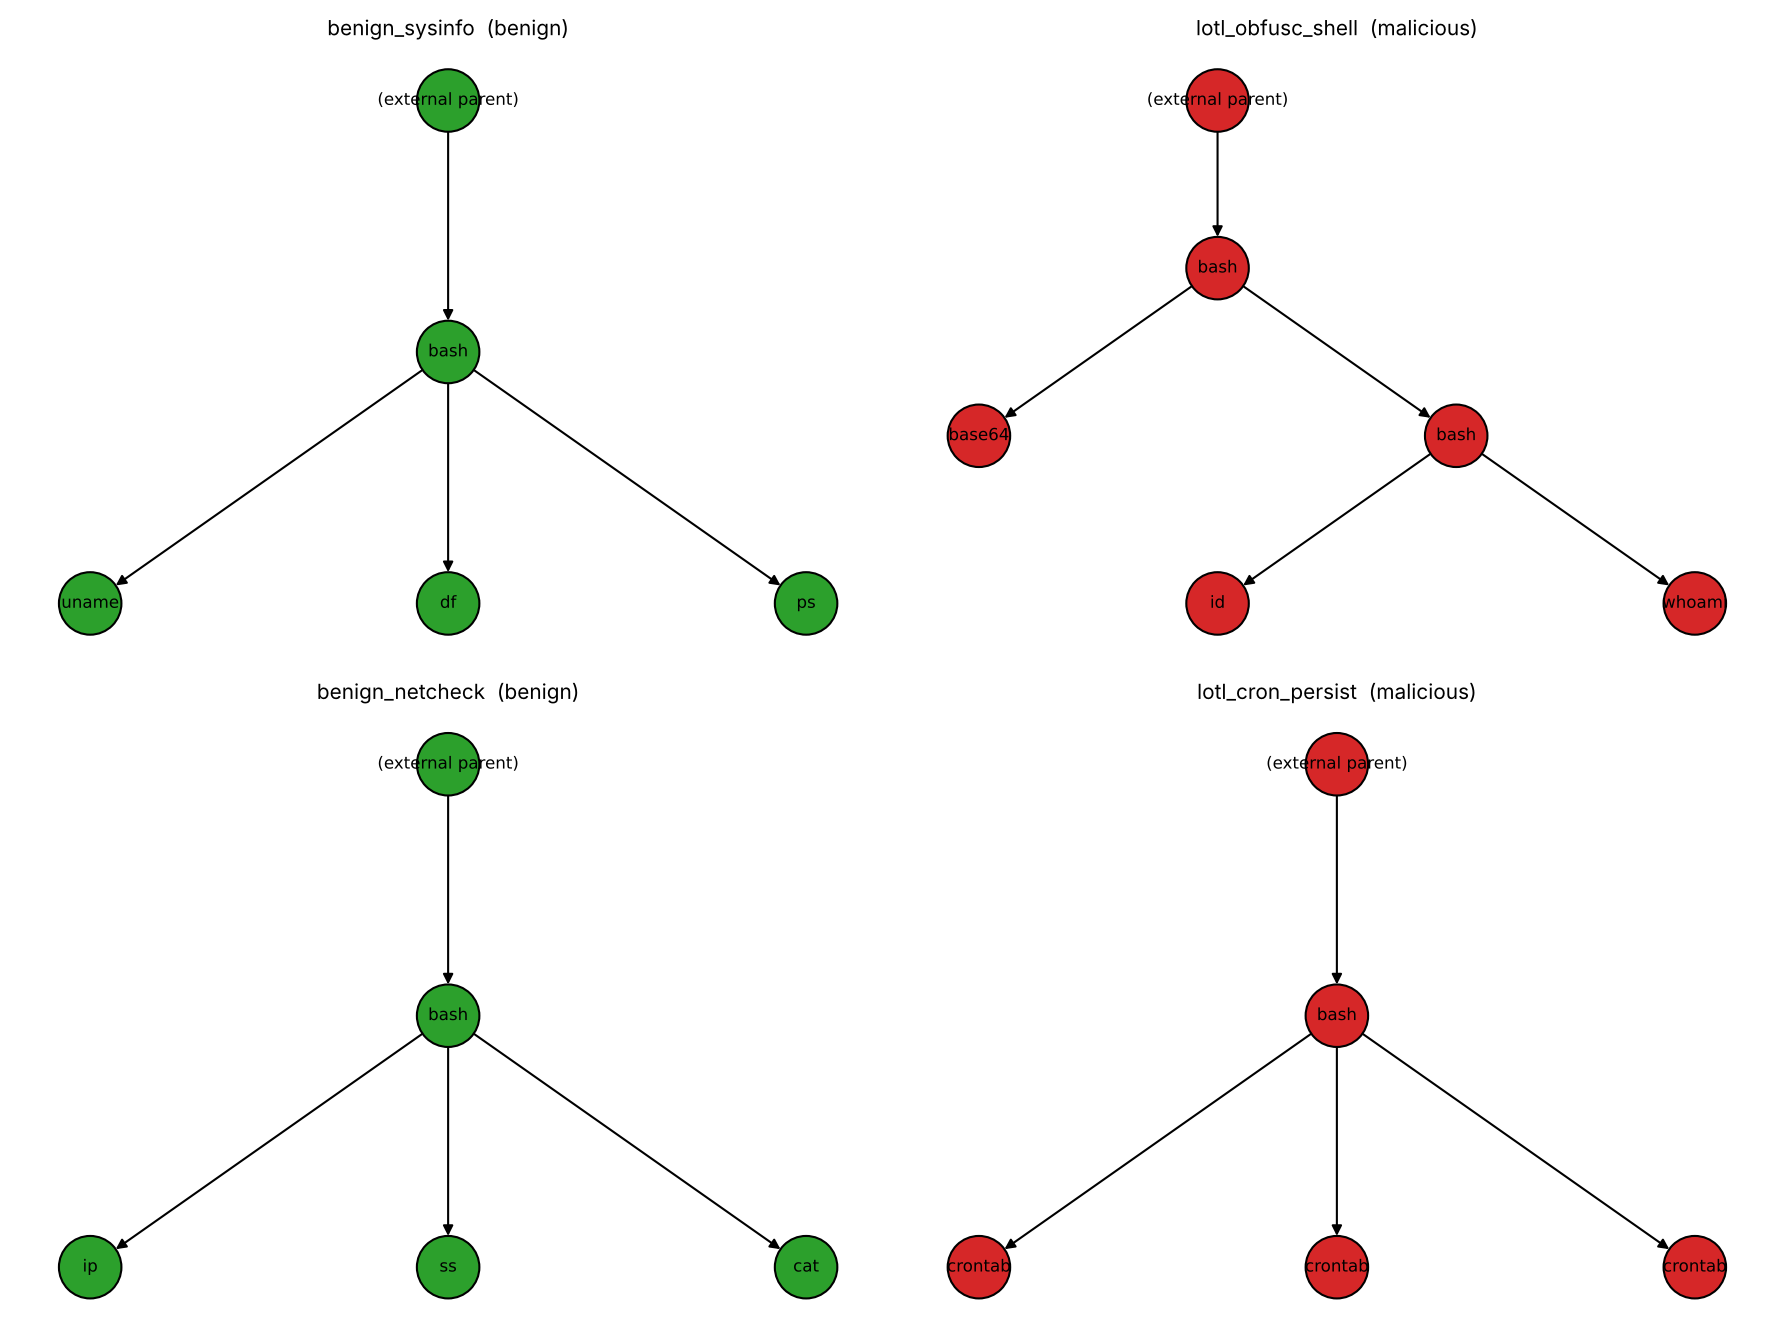
\includegraphics[width=\columnwidth]{fig_provenance_graphs.png}
\caption{Process-provenance graphs. Benign administrative tasks (left, green)
produce shallow fan-outs from a single shell; emulated LotL activities
(right, red) produce deeper or atypical chains using the same trusted
binaries.}
\label{fig:graphs}
\end{figure}

\begin{figure}[htbp]
\centering
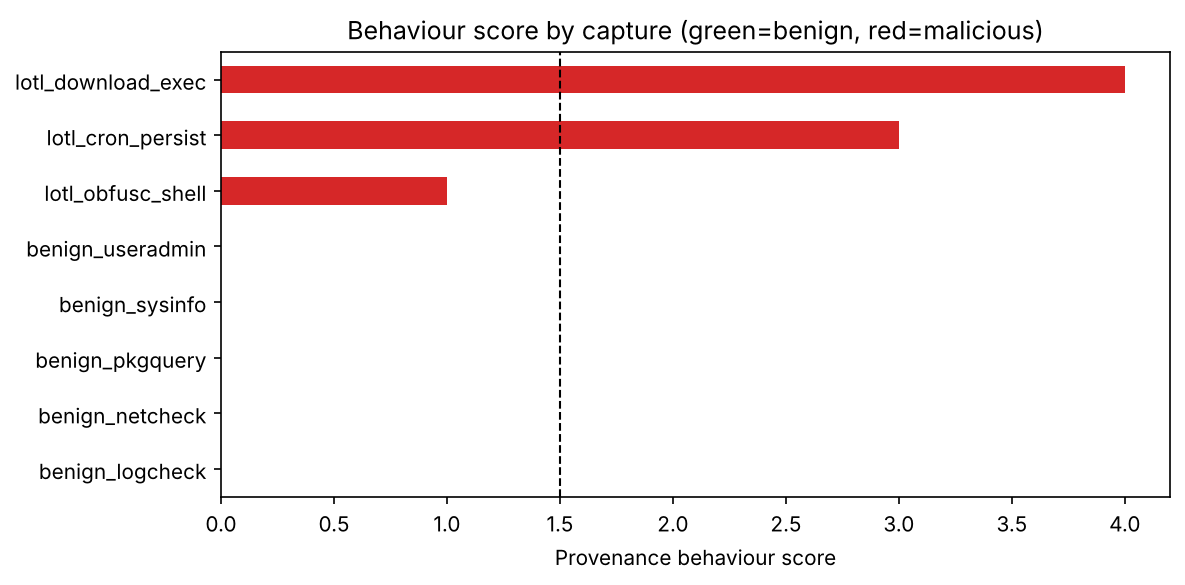
\includegraphics[width=\columnwidth]{fig_scores.png}
\caption{Provenance behaviour score per capture. The dashed line is the
decision threshold; benign activities fall below it while emulated LotL
activities rise above.}
\label{fig:scores}
\end{figure}

\subsection{Comparative Analysis and Interpretation}
% >>> WRITE IN YOUR OWN WORDS, using YOUR numbers. Key point to make:
% The name-based baseline attains perfect recall but low precision because it
% flags benign administrative use of bash/curl/crontab, i.e., false positives.
% The provenance score removes those false positives by using behavioural
% context, trading a small amount of recall for a large precision gain. Note
% any technique the score currently misses and why (motivates future work).

\subsection{Limitations and Planned Work}
This is a controlled, small-sample Linux prototype with a rule-based score;
results are indicative rather than conclusive. Planned work for the final
report includes scaling the dataset, adding the Windows/Sysmon half, training
and cross-validating a supervised model, and evaluating robustness under
additional obfuscation and detection latency.

%---------------------------------------------------------------------
\bibliographystyle{IEEEtran}
\bibliography{references}

\end{document}
